\section{Identification of the boat parameters}
The aim of this section is to use basic identification techniques of system parameters that are not explicity given by the system model.

\subsection{Problem a}

To calculate the transfer function from $\delta$ to $\psi$, assuming no disturbances($w_w = w_b = 0$), we use the method that you see below. The transfer function $H_{ship}(s)$, parametrized by $T$ and $K$, can be stated as done in \cref{eq:H_ship}.


From \cref{eq:ship_model_psi}-(\ref{eq:ship_model_b}) we get \cref{eq:from_model_to_H_ship}:

\begin{subequations} \label{eq:from_model_to_H_ship}
    \begin{align}
    \dot{\psi} &= r \\ 
    \dot{r} &= - \frac{1}{T} r + \frac{K}{T} (\delta - b) \\
    b &= w_b
    \end{align}
\end{subequations}

Rearranging the equations in \cref{eq:from_model_to_H_ship}, we can state it as \cref{eq:psi_ddot}:

\begin{equation} \label{eq:psi_ddot}
    \ddot{\psi} = - \frac{1}{T} \dot{\psi} + \frac{K}{T} (\delta - 0)
\end{equation}

We then Laplace transform it and reorganize the terms to give us \cref{eq:H_ship}:

\begin{equation} \label{eq:H_ship}
    \frac{\psi(s)}{\delta(s)} = H_{ship}(s) = \underline{\frac{K}{s^2 T + s}}
\end{equation}

\subsection{Problem b}\label{sec:boat_param_calm}

We want to identify the boat paramaters $T$ and $K$ in calm weather, with no wave or current disturbance. Running the simulation with sine inputs with amplitude 1 and frequencies $\omega_1 = 0.005$ and $\omega_2 = 0.05$ gives a set of equations to derive $T$ and $K$ from. We used the peak to peak analyzer in the Simulink scopes for the amplitude of the output in both problem b) and c) below. The plot of these responses can be seen labeled as "Calm weather" in \cref{fig:p5p1_0.005} and \cref{fig:p5p1_0.05} respectively. The amplitude values for calm weather are stated in \cref{eq:amplitudes}.

\begin{figure}[h]
	\centering
	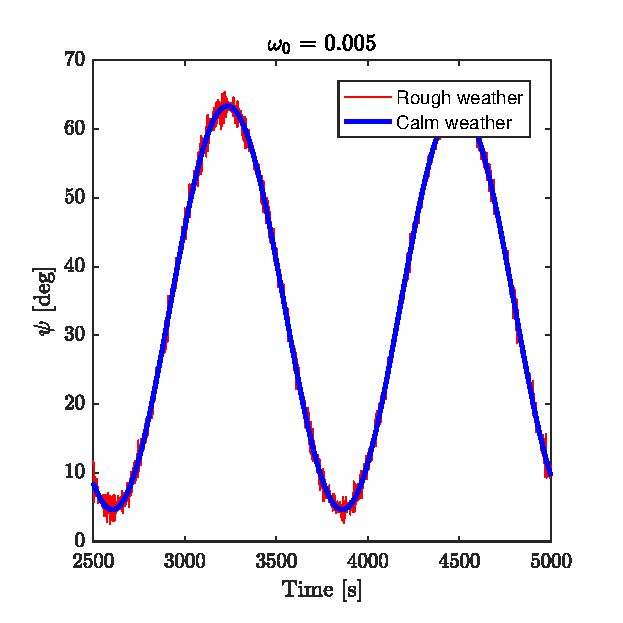
\includegraphics[width=\textwidth]{figures/Ass1_omega_005.eps}
	\caption{Compass measurement}
\label{fig:p5p1_0.005}
\end{figure}

\begin{figure}[h]
	\centering
	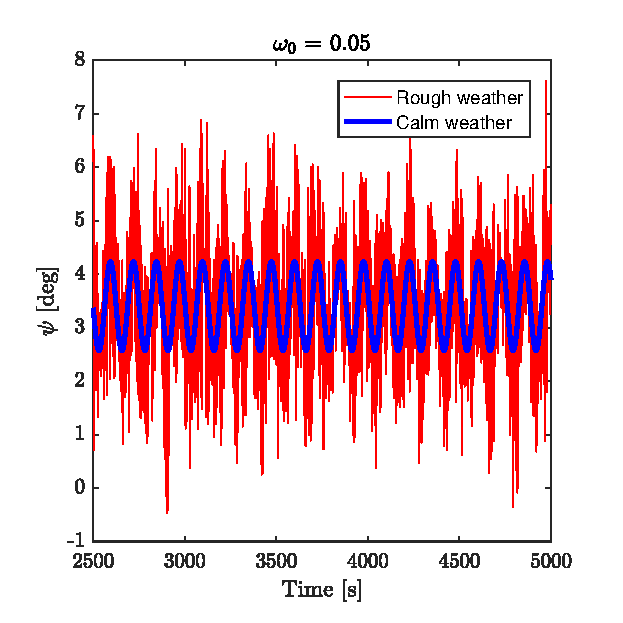
\includegraphics[width=\textwidth]{figures/Ass1_omega_05.eps}
	\caption{Compass measurement}
\label{fig:p5p1_0.05}
\end{figure}

\begin{equation}\label{eq:amplitudes}
    H_1 = |H(j \omega_1)| = 29.36,
    \quad
    H_2 = |H(j \omega_2)| = 0.831
\end{equation}

this gives us the the set of equations in \cref{eq:ampl_eq}

\begin{subequations}\label{eq:ampl_eq}
    \begin{align}
        H_1^2 (\omega_1^4 T^2 + \omega_1^2) - K^2 &= 0 \\
        H_2^2 (\omega_2^4 T^2 + \omega_2^2) - K^2 &= 0
    \end{align}
\end{subequations}

Solving \cref{eq:ampl_eq} allows us to determine $T$ and $K$ and their values can be seen in \cref{eq:T_and_K}.

\begin{subequations} \label{eq:T_and_K}
    \begin{align}
        T &= \sqrt{\frac{H_1^2 \omega_1^2 - H_2^2 \omega_2^2}{H_2^2 \omega_2^4 - H_1^2 \omega_1^4}} = \underline{72.44} \label{eq:T} \\
        K &= \sqrt{H_1^2 (\omega_1^4 T^2 + \omega_1^2)} = \underline{0.156} \label{eq:K}
    \end{align}
\end{subequations}





\subsection{Problem c}

We repeat the process from \cref{sec:boat_param_calm} with waves and measurement noise on. The responses are again in \cref{fig:p5p1_0.005} and \cref{fig:p5p1_0.05} and we now examine the plots labeled "Rough weather". The extracted amplitudes are given by \cref{eq:ampl_rough}.

\begin{equation}\label{eq:ampl_rough}
    H_1 = |H(j \omega_1)| = 31.145,
    \quad
    H_2 = |H(j \omega_2)| = 4.0435
\end{equation}

Inserting these amplitudes into \cref{eq:T_and_K} gives us an estimate for boat parameters given by \cref{eq:T_and_K_rough} which are not a good estimate of the boat parameters.

\begin{equation}\label{eq:T_and_K_rough}
    T = i12.79, 
    \quad
    K = 0.156
\end{equation}

We see that the results for rough weather in \cref{fig:p5p1_0.005} and \cref{fig:p5p1_0.05} are heavily influenced by the disturbances and noise, especially the signal with input frequency $\omega_2 = 0.05$ as seen in \cref{fig:p5p1_0.05}. This makes our estimates poor because it's very hard to accurately determine an amplitude on the signal mentioned above. Even though we get the same $K$, $T$ is estimated to be imaginary.

\subsection{Problem d}
We want to examine if our boat parameters are reasonable by comparing our theoretical model, \cref{eq:H_ship}, and the simulated step response of the cargo-ship. We do this by implementing our transfer function in Simulink, and giving both it and the cargo-ship the same step input and plot them side-by-side. The simulink implementation for this is seen in \cref{fig:p5p1d_model} in \cref{sec:simulink}.

Applying a step input of $1^\circ$ on the rudder gives us the step response shown in \cref{fig:p5p1d_step_response}. As can be seen, the values for $T$ and $K$ are pretty good as the step response of the model follows the response of the ship with an acceptably small error.


\begin{figure}[h]
	\centering
	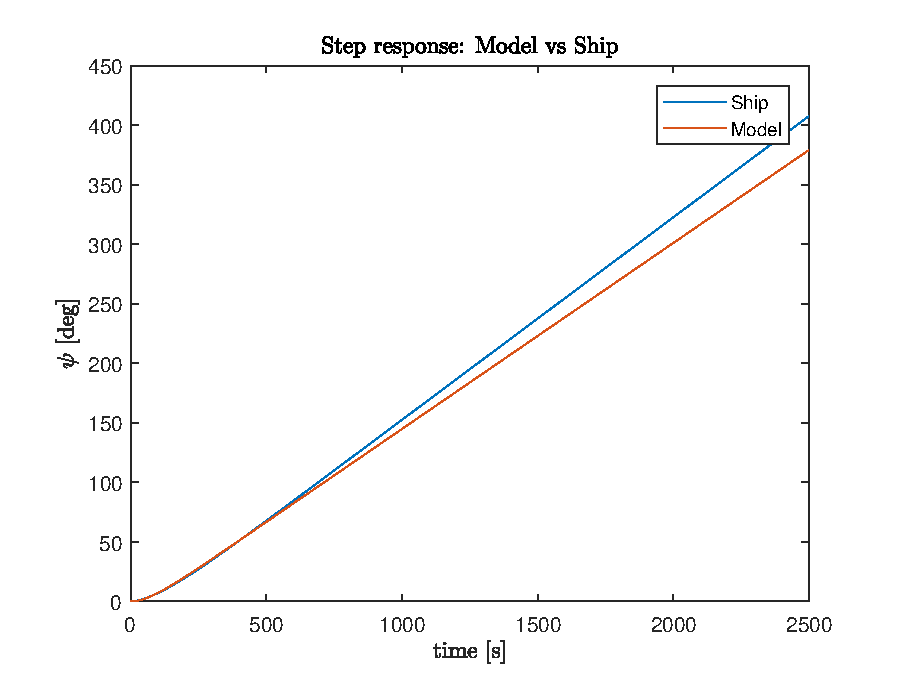
\includegraphics{figures/p5p1d.eps}
	\caption[width=\textwidth]{Step response of ship and theoretical model}
\label{fig:p5p1d_step_response}
\end{figure}

We also note that our estimation of the boat parameters $T$ and $K$ could be improved. There is a growing discrepancy between our modeled response and the actual cargo-ship simulation. One main cause of this discrepancy is our method of finding the signal amplitude. We use a pretty naive method of just reading the peak-to-peak values of our output in a small interval. Increasing this interval by running the simulation longer or use a better procedure for amplitude extraction will yield more accurate estimates for the boat parameters. However we deem the results good enough to move on with the Kalman filtering.

\\\\

In all the following parts of this report measurement noise will be turned on in the ship model when running the simulations.
